% HW Template for CS 6150, taken from https://www.cs.cmu.edu/~ckingsf/class/02-714/hw-template.tex
%
% You don't need to use LaTeX or this template, but you must turn your homework in as
% a typeset PDF somehow.
%
% How to use:
%    1. Update your information in section "A" below
%    2. Write your answers in section "B" below. Precede answers for all 
%       parts of a question with the command "\question{n}{desc}" where n is
%       the question number and "desc" is a short, one-line description of 
%       the problem. There is no need to restate the problem.
%    3. If a question has multiple parts, precede the answer to part x with the
%       command "\part{x}".
%    4. If a problem asks you to design an algorithm, use the commands
%       \algorithm, \correctness, \runtime to precede your discussion of the 
%       description of the algorithm, its correctness, and its running time, respectively.
%    5. You can include graphics by using the command \includegraphics{FILENAME}
%
\documentclass[11pt]{article}
\usepackage{amsmath,amssymb,amsthm}
\usepackage{graphicx}
\usepackage[margin=1in]{geometry}
\usepackage{fancyhdr}
\usepackage{algorithm}
\usepackage{algpseudocode}
\usepackage{pifont}
\setlength{\parindent}{0pt}
\setlength{\parskip}{5pt plus 1pt}
\setlength{\headheight}{13.6pt}
\newcommand\question[2]{\vspace{.25in}\hrule\textbf{#1: #2}\vspace{.5em}\hrule\vspace{.10in}}
\renewcommand\part[1]{\vspace{.10in}\textbf{(#1)}}
\newcommand\algorith{\vspace{.10in}\textbf{Algorithm: }}
\newcommand\correctness{\vspace{.10in}\textbf{Correctness: }}
\newcommand\runtime{\vspace{.10in}\textbf{Running time: }}
\pagestyle{fancyplain}
\lhead{\textbf{\NAME\ (\UID)}}
\chead{\textbf{HW\HWNUM}}
\rhead{CS 6350, \today}
\begin{document}\raggedright
%Section A==============Change the values below to match your information==================
\newcommand\NAME{Jake Pitkin}  % your name
\newcommand\UID{u0891770}     % your utah UID
\newcommand\HWNUM{4}              % the homework number
%Section B==============Put your answers to the questions below here=======================

\question{1}{PAC Learning}

\textbf{Rule 1:} You are free to combine any of the parts as they are.

\textbf{Rule 2:} You may also cut any of the parts into two distinct pieces before using them.

\part{1a} Given $N$ parts, each product that can be made out of these parts is a distinct hypothesis $h$ in the hypothesis space $H$. From \textit{Rule 1}, a worker can choose to include or not include any of the parts in a product. This can be viewed as a monotone conjunction as a product is defined by choosing to include or not include each of the $N$ parts. There exists $2^N$ possible products as there are two choices for each of the $N$ parts. We will not consider the product constructed by using none of the parts.
	
	\framebox[1.2\width]{$|H| = 2^N - 1$}

\part{1b} The experienced worker now creates a product using \textit{Rule 1} and \textit{Rule 2}. There are now four choices that can be made for each of the parts: don't include it, include it, cut the part and use the first half or cut the part and use the second half. A product is now defined as making four choices for each of the $N$ parts. Thus there are $4^N$ possible products. We will not consider the product constructed by using none of the parts.

	\framebox[1.2\width]{$|H| = 4^N - 1$}

\part{1c} By applying the principles of Occams's Razor we can make a statement about the number of required examples the robot will have to see to have an error of 0.01 with probability $99\%$ on products with 6 available parts.

Given a hypothesis space $H$, we can say with probability $1 - \delta$, a hypothesis $h \in H$, that is consistent with a training set of size $m$, will have an error $< \epsilon$ on future examples if

$$m > \frac{1}{\epsilon}(ln(|H|) + ln\frac{1}{\delta})$$

We want an error rate of $\epsilon = 0.01$ with probability $1 - \delta = 0.99$ with a $|H| = 4^6 = 4,096$.

$$m > \frac{1}{0.01}(ln(4,095) + ln\frac{1}{0.01})$$
$$m > 1,292.27$$

The robot will have to see at least $1,293$ examples to guarantee a $0.01$ error with probability $99\%$ if there are 6 available parts. We round up as the number of required examples must be an integer value and rounding down would not satisfy the equality. We can use this inequality as we know the true function is contained inside the hypothesis space.

\framebox[1.2\width]{at least 1,293 examples}
\newpage
\part{2} The Chernoff bounds govern the probability that $S/m$ will differ from $p$ by some factor $0 \leq \gamma \leq 1$.
	$$Pr[S/m > (1 + \gamma)p] \leq e^\frac{-mp\gamma^2}{3}$$	
	$$Pr[S/m < (1 - \gamma)p] \leq e^\frac{-mp\gamma^2}{2}$$	
	
$\mathbf{error_s(h)}$: the sum S of the independent errors made over $m$ examples by some hypothesis $h$. This is the observed error of $h$ and is equivalent to $S/m$.

$\mathbf{error_d(h)}$: the true error or generalization error. This is equivalent to the expected value of $S/m$ or $E[S/m] = p$. Since the distribution is i.i.d, if we see a sufficient number of consistent examples the true error will be no worst than the observed error plus some $\epsilon$ with probability $1 - \delta$. Where $0 \leq \epsilon, \delta \leq 1$.
	
We want the probability there exists a $h \in H$ whose $error_s(h)$ differs from $error_d(h)$ by at most $\epsilon$.
$$Pr[\exists h; S/m > (1 + \gamma)p] \leq |H|e^\frac{-mp\gamma^2}{3}$$
This probability must be bounded above by a $\delta$ value. I choose the Chernoff bound I did as it will give a tighter bound than the other choice.
$$Pr[\exists h; S/m > (1 + \gamma)p] \leq |H|e^\frac{-mp\gamma^2}{3} \leq \delta$$
We want to isolate $m$ on one side of inequality to analyze the minimum number of required consistent examples needed.
$$|H|e^\frac{-mp\gamma^2}{3} \leq \delta$$
$$\frac{|H|}{e^{\frac{mp\gamma^2}{3}}} \leq \delta$$
$$|H| \leq \delta *e^{\frac{mp\gamma^2}{3}}$$
$$\frac{|H|}{\delta} \leq e^{\frac{mp\gamma^2}{3}}$$
$$ln(\frac{|H|}{\delta}) \leq ln(e^{\frac{mp\gamma^2}{3}})$$
$$ln(|H|) - ln(\delta) \leq \frac{mp\gamma^2}{3}$$
$$\frac{3}{p\gamma^2}[ln(|H|) - ln(\delta)] \leq m$$

\framebox[1.2\width]{$ m \geq \frac{3}{p\gamma^2}[ln(|H|) + ln(\frac{1}{\delta})]$}

We want to bound the number of required examples needed in terms of $\epsilon$ and not $\gamma$. To resolve this we will find a relationship between $\epsilon$ and $\gamma$. 

Recall we want to ensure every hypothesis will have true error no worse than $(1 + \epsilon)error_s(h)$ with a probability less than $\delta$. We showed true error or $error_d(h)$ is $p$ and $error_x(h)$ is $\frac{S}{m}$.

$$Pr[p  > (1 + \epsilon) \frac{S}{m}] \leq \delta$$

Comparing this to one of the provided Chernoff bounds, we can find a relationship between $\epsilon$ and $\gamma$.

$$Pr[\frac{S}{m} < (1 - \gamma)p] \leq e^{\frac{-mp\gamma^2}{2}} \leq \delta$$
$$Pr[p > \frac{1}{(1 - \gamma)}\frac{S}{m}] \leq \delta$$

We can see that $(1 + \epsilon)$ and $1 \backslash (1 - \gamma)$ are equal by rearranging terms and comparing the two probabilities. We want to replace $\gamma$ with an expression containing $\epsilon$, so we isolate $\gamma$.

$$\gamma = 1 - \frac{1}{(1 + \epsilon)}$$

We want $0 \leq \epsilon \leq 1$, to achieve this we bound $\gamma$ as $0 \leq \gamma \leq 0.5$. Finally, we replace $\gamma$ in the inequality from above with the equivalent expression containing $\epsilon$.

$$ m \geq \frac{3}{p\gamma^2}[ln(|H|) + ln(\frac{1}{\delta})]$$
$$ m \geq \frac{3}{p(1 - \frac{1}{1 + \epsilon})^2}[ln(|H|) + ln(\frac{1}{\delta})]$$
$$ m \geq \frac{3}{\frac{p\epsilon^2}{(\epsilon + 1)^2}}[ln(|H|) + ln(\frac{1}{\delta})]$$
$$ m \geq \frac{3(\epsilon + 1)^2}{p \epsilon^2}[ln(|H|) + ln(\frac{1}{\delta})]$$

This concludes the derivation of the number of training examples sufficient to make $\epsilon$ and $\gamma$ guarantees for a given $|H|$.

\framebox[1.2\width]{$ m \geq \frac{3(\epsilon + 1)^2}{p \epsilon^2}[ln(|H|) + ln(\frac{1}{\delta})]$}

\question{2}{VC Dimensions}
\textbf{Shatter:} A set of examples S is \textit{shattered} by a set of functions H if for every partition of the examples in S into positive and negative examples there is a function in H that gives exactly these labels to the examples.

\textbf{VC Dimension:} The \textit{VC Dimension} of hypothesis space H over instance space X is the size of the largest finite subset of X that is shattered by H.

\part{1} We want to prove that a finite hypothesis space $\mathcal{C}$ has a VC dimension at most $log_2|\mathcal{C}|$. That is, $VC(\mathcal{C}) \leq log_2|\mathcal{C}|$.

\textbf{Proof by contradiction:} Assume that the opposite $VC(\mathcal{C}) > log_2|C|$ is true.

Take a finite instance space X of size d. There exists $2^d$ (the number of possible binary vectors of length $d$) ways to partition X. Thus the  $\mathcal{|C|} = 2^d$.

Given that X is of size d, it holds that $0 \leq VC(C) \leq d$ as $\mathcal{C}$ can shatter \textbf{at most} d points (the size of the instance space). Visiting the initial assumption:

$$VC(\mathcal{C}) > \log_2|C|$$
$$VC(\mathcal{C}) > d$$

Arriving at the contradiction $0 \leq VC(\mathcal{C}) \leq d$ and $VC(\mathcal{C}) > d$. Thus proving $VC(\mathcal{C}) \leq log_2|\mathcal{C}|$.

\part{2} For part a and b of this question, consider only $k$ such that $|X| > k$ by a considerable amount, as per the announcement by Jie Cao to simplify this question. 

\part{2a} The proof for the VC dimension of $\mathcal{H}$ involves two parts. First, we must show that there \textit{exists} any subset of size $d$ that can be shattered (this proves $VC(\mathcal{H}) \geq d$). Second, we must show that \textit{no subset} of size d can be shattered by $\mathcal{H}$ (this proves $VC(\mathcal{H}) < d$). The result of these two bounding inequalities proves $VC(\mathcal{H}) = d$.

\textbf{Proof} (1) To prove $VC(\mathcal{H}) \geq k$ we must give one example of $k$ points in $\mathcal{X}$ that can be shattered by $\mathcal{H}$. We know that every $h \in \mathcal{H}$ is a vector of length $|X|$ containing $k$ 1's and $|X| - k$ 0's. More so, $\mathcal{H}$ contains every permutation of $k$ 1's and $|X| - k$ 0's. Allowing $\mathcal{H}$ to shatter an example of size $k$ as $\mathcal{H}$ contains hypotheses that gives all possible labelings of the $k$ examples.

	The typical labelings are as such. Labeling all examples as + can be accomplished as we have all permutations of k 1's. Assuming k is must smaller than $|X|$ we also have all permutations of at least k 0's. All other labelings follow similar logic: the desired hypothesis will satisfy exactly k 1's.

(2) To prove $VC(\mathcal{H}) < k + 1$ we must show that any set of $k + 1$ points can't be shattered by $\mathcal{H}$. To show this, for any set of $k + 1$ points we assign a positive label to all of them. $\mathcal{H}$ doesn't contain a function to partition these examples properly as all $h \in \mathcal{H}$ are a vector of length $|X|$ containing exactly $k$ 1's. Thus we have proven $VC(\mathcal{H}) = k$.

\framebox[1.2\width]{$VC(\mathcal{H}) = k$}

\part{2b} {Proof} (1) To prove $VC(\mathcal{H}) \geq 2k + 1$ we must give one example of $2k + 1$ points in $\mathcal{X}$ that can be shattered by $\mathcal{H}$. Each $h \in \mathcal{H}$ contains at most $k$ 1's or $k$ 0's. $\mathcal{H}$ is composed of every permutation of vectors containing at most $k$ 1's or $k$ 0's. Therefore, it will be able to shatter an example of $2k + 1$ as for any labeling of the examples, $\mathcal{H}$ can produce a hypothesis that splits them as such. 

	The typical labelings are as such. Labeling all examples + can be accomplish with zero 0's and the rest 1's, similarly all examples can be labeled - with zero 1's and the rest 0's. The hardest labeling is k 1's and k + 1 0's, or vice versa. This can be accomplish though as at least one of the constraints is met. All other labelings following similar logic: at least one constraint can be made true.

(2) To prove $VC(\mathcal{H}) < 2k + 2$ we must show that any set of $2k + 2$ points can't be shattered by $\mathcal{H}$. To show this, for any set of $2k + 2$ points we assign a positive label to $k + 1$ and a negative label to the other $k + 1$. $\mathcal{H}$ does not contain an $h$ such that $k + 1$ entries are 1's and $k + 1$ are 0's as this doesn't satisfy either constraint. Thus we have proven $VC(\mathcal{H}) = 2k + 1$.

\framebox[1.2\width]{$VC(\mathcal{H}) = 2k + 1$}

\part{3} \textbf{Proof} (1) To prove $VC(\mathcal{H}) \geq 4$ we must give one example of points $x_1, x_2, x_3, x_4 \in \mathbb{R}$ that can be shattered by $\mathcal{H}$. Take the points $x_1 = 1$, $x_2 = 2$, $x_3 = 3$, and $x_4 = 4$. There are 16 possible labelings of the four points and we must show there is a $h \in \mathcal{H}$ that satisfies each labeling. The figure below expresses all the possible labelings, excluding labelings that are symmetric to provided labelings to avoid an excessiveness of figures.

\begin{figure}[H]
  \centerline{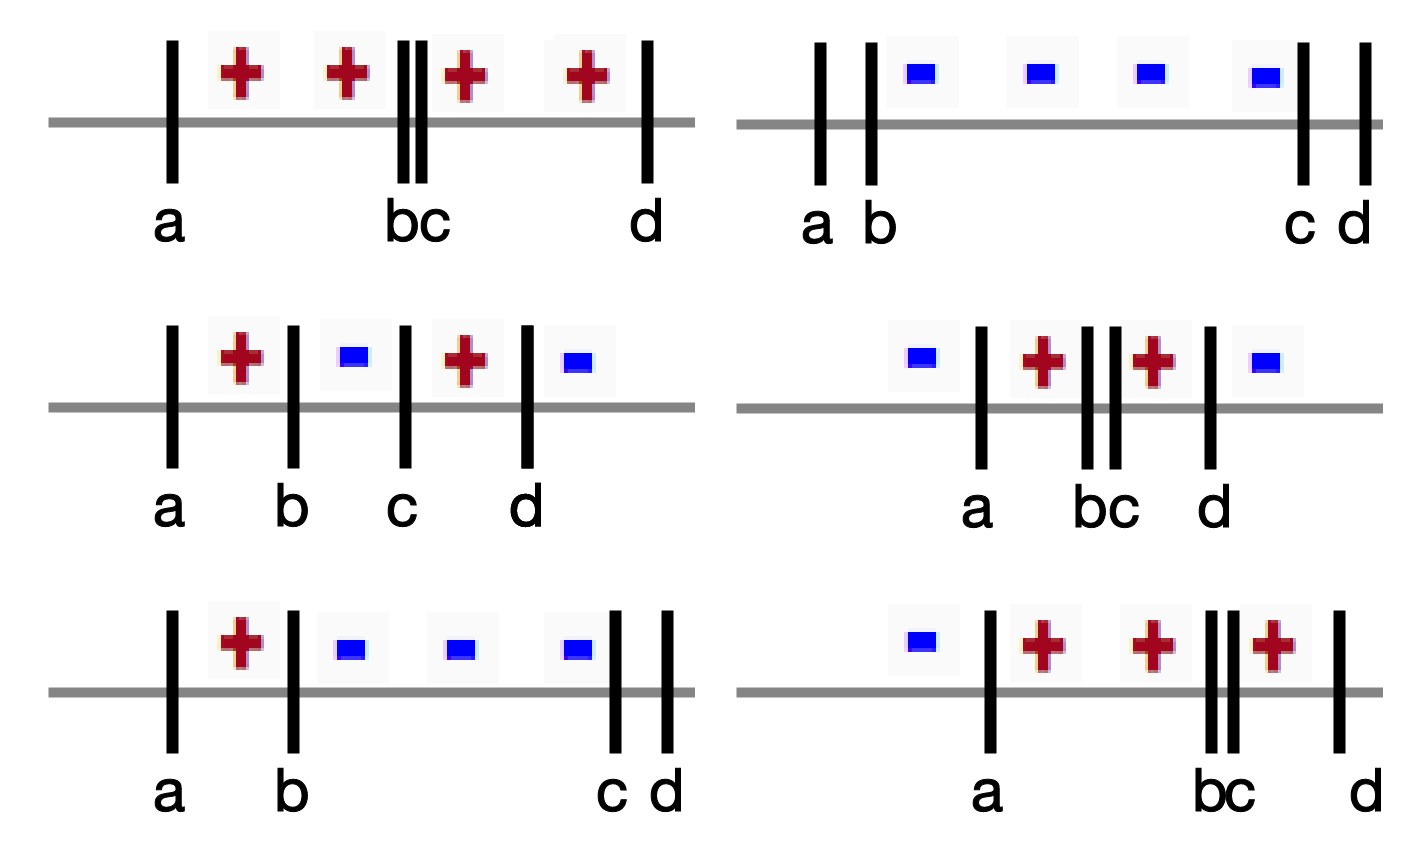
\includegraphics[width=0.5\linewidth]{image_2_3_1.png}}
  \caption{Labeling of four example points and a $h \in \mathcal{H}$ that shatters each of them.}
\end{figure}

This proves $VC(\mathcal{H}) \geq 4$. (2) To prove $VC(\mathcal{H}) < 5$, we must prove there doesn't exist a set of \textbf{any} five points that can be shattered by $\mathcal{H}$. Given \textbf{any} five unique points $x_i \in \mathbb{R}$, there exists a labeling s.t. $\mathcal{H}$ cannot shatter the set of five points.

\begin{figure}[H]
  \centerline{
\includegraphics[width=0.5\linewidth]{image_2_3_2.png}}
  \caption{Labeling of five points that can not be shattered by $\mathcal{H}$}
\end{figure}

There exists the relationship $x_i < x_j < x_k < x_l < x_m$. That is, choosing any five real numbers, they can be arranged to satisfy the inequality. Starting with $x_i$, label it positive and alternate labelings moving along the five points in ascending order. There is no way to shatter these labeled five points with $\mathcal{H}$. Thus we have proven the $VC(\mathcal{H}) = 4$.

\framebox[1.2\width]{$VC(\mathcal{H}) = 4$}

\part{4} \textbf{Proof} (1) To prove $VC(H) \geq 2$ we must give one example of two points $\mathbf{x_1}, \mathbf{x_2} \in \mathbb{R}^2$ that can be shattered by $H$. Take the points $\mathbf{x_1} = \{-1, 1\}$ and $\mathbf{x_2} = \{1, 1\}$. There are four possible labelings of the two points and we must show there is a $h \in H$ that satisfies each labeling.

\begin{figure}[H]
  \centerline{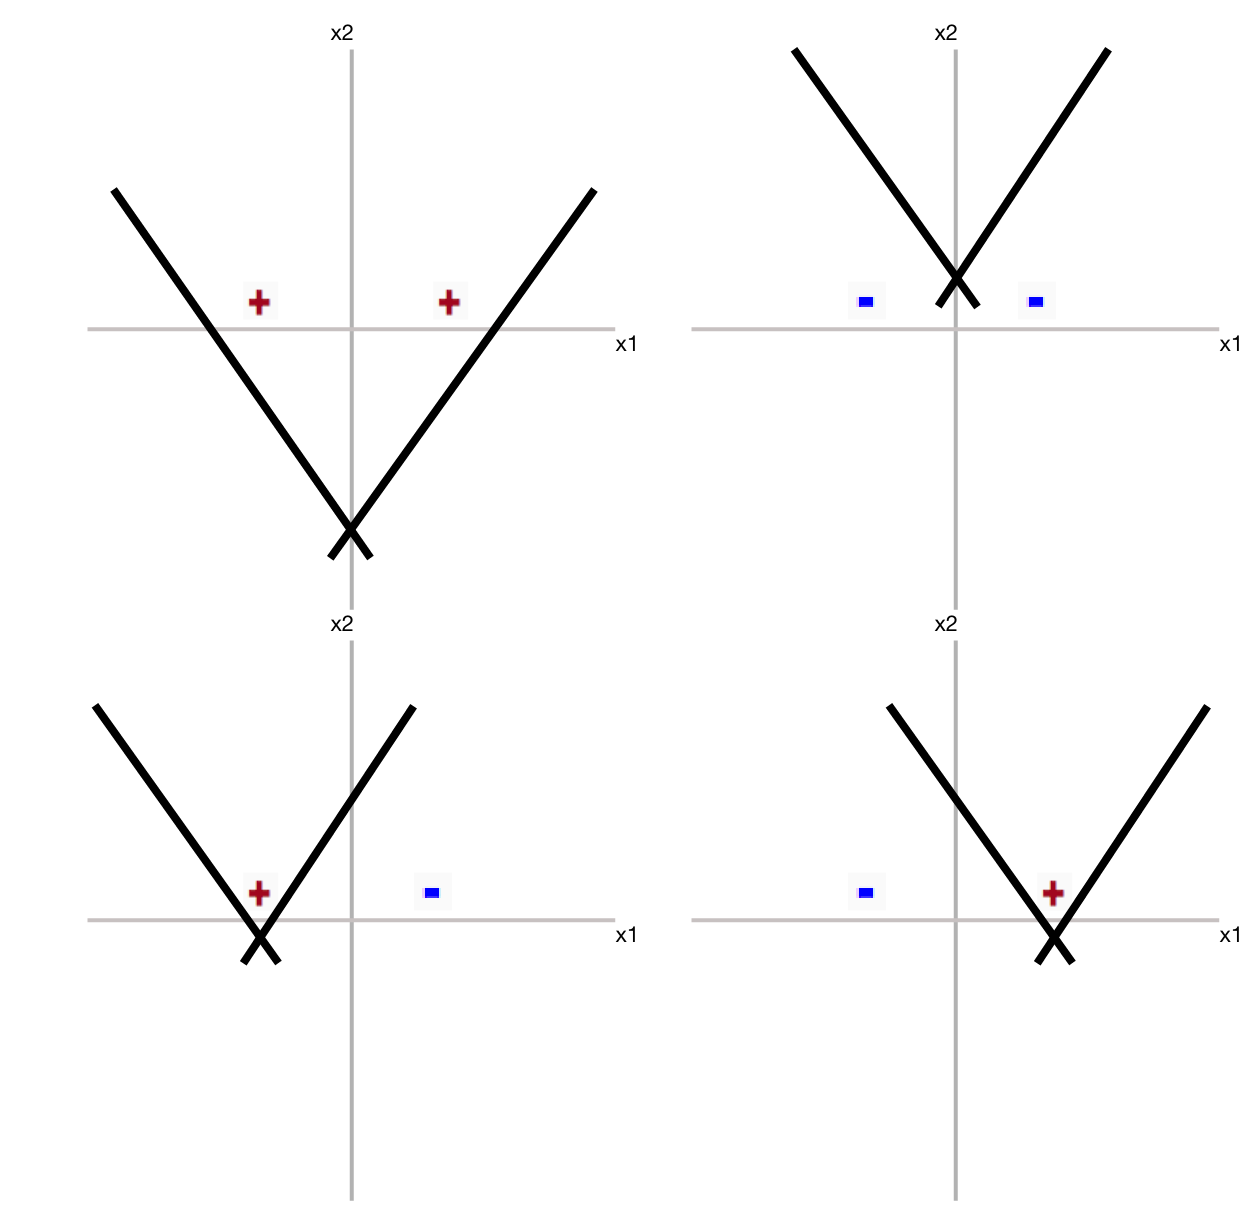
\includegraphics[width=0.5\linewidth]{image_2_4_1.png}}
  \caption{Labeling of two example points and a $h \in \mathcal{H}$ that shatters each of them.}
\end{figure}

 \begin{table}[H]
\centering
{\renewcommand{\arraystretch}{1.2}%
\begin{tabular}{| c | c | c | c |}
\hline
$\mathbf{x_1} \ label$& $\mathbf{x_2} \ label$ & $a$ & $b$\\
\hline
+ & + & -4 & 4\\ \hline
- & - & 4 & -4\\ \hline
+ & - & 0& -2 \\ \hline
- & + & 2 & 0\\ \hline
\end{tabular}}
\caption{a and b values that define a $h \in H$ that shatter each labeling.}
\end{table}

This proves $VC(H) \geq 2$. (2) To prove $VC(H) < 3$, we must prove there doesn't exist a set of three points that can be shattered by H. Given \textbf{any} three unique points $\mathbf{x} \in \mathbb{R}^2$, there exists a labeling s.t. $H$ cannot shatter the set of three points.

When selecting three points in $\mathbb{R}^2$ we can choose the points to be in a vertical line, a horizontal line, or form the corners of a triangle.

\begin{figure}[H]
  \centerline{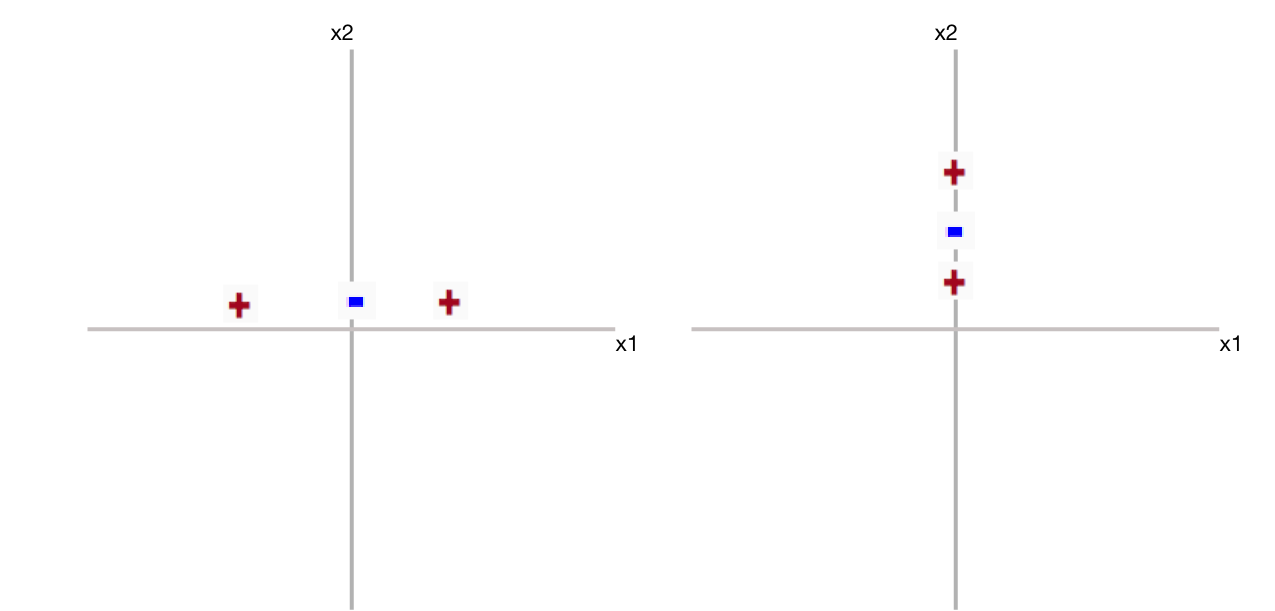
\includegraphics[width=0.5\linewidth]{image_2_4_2.png}}
  \caption{Collinear labelings that can't be shattered by $H$.}
\end{figure}

We can clearly see that $H$ cannot shatter these points.

\begin{figure}[H]
  \centerline{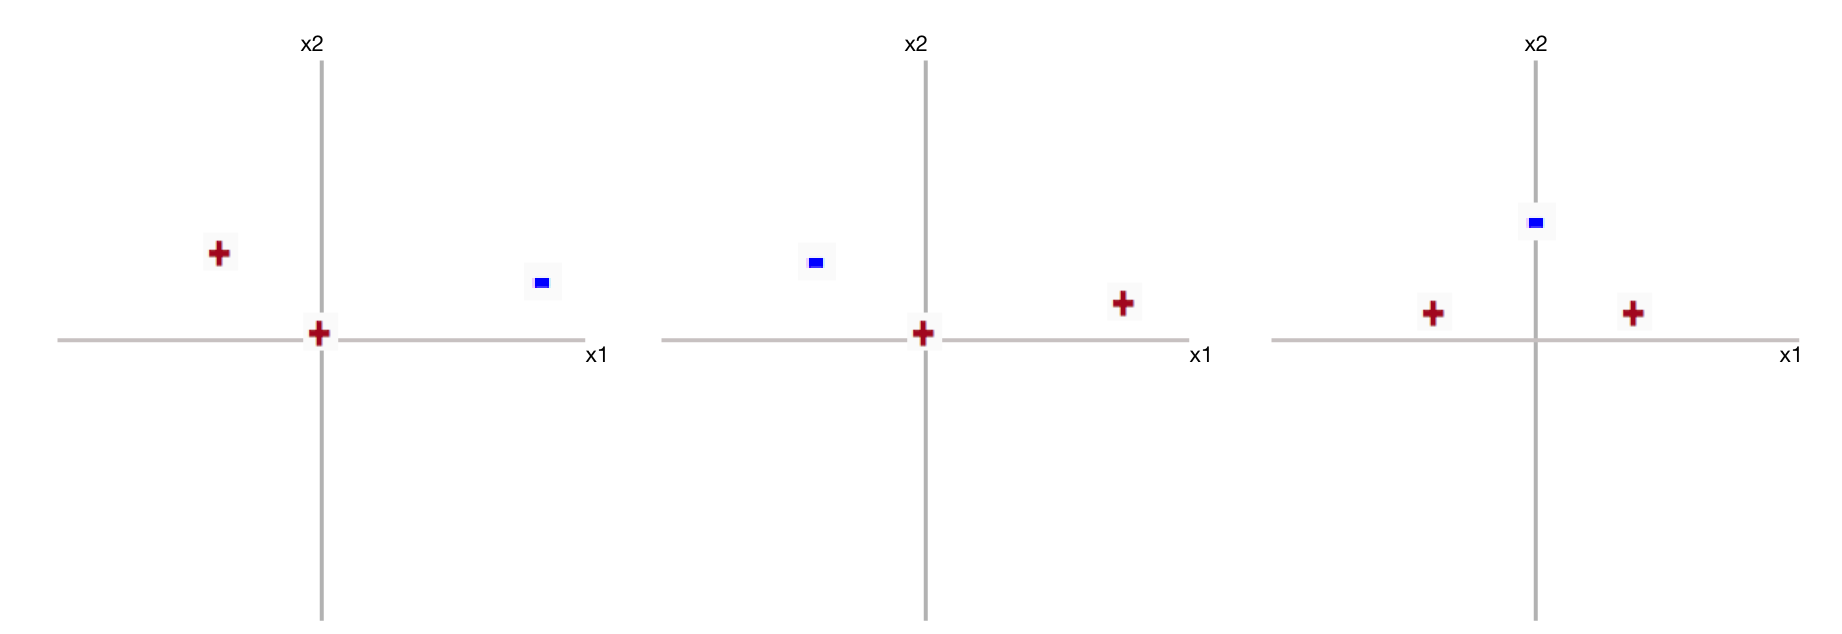
\includegraphics[width=0.8\linewidth]{image_2_4_3.png}}
  \caption{Triangular assignments that can't be shattered by $H$.}
\end{figure}

The first two examples are the same set of points with two different labelings. There exists a $h \in H$ that can split the first labelings, but not the second labelings. This example is symmetrical: we can shift one point far from the other two to satisfy one labeling but in the process makes another labeling impossible to split with H.

The third example shows that the option of raising the middle point above the other two points also can't be separated.

Thus, there is no set of three points that can be shattered by $H$, proving $VC(H) < 3$.

We now know $VC(H) \geq 2$ and $VC(H) < 3$, proving $VC(H) = 2$.

\framebox[1.2\width]{$VC(H) = 2$} 

\part{5} Let two hypothesis classes $H_1$ and $H_2$ satisfy $H_1 \subseteq H_2$. Prove: $VC(H_1) \leq VC(H_2)$.

\textbf{Proof by contradiction:} Assume that the opposite $VC(H_1) > VC(H_2)$ is true.

Let X be a finite instance space and $VC(H_1) = d$. That is, a set of examples S of size d are shattered by $H_1$. Meaning for every partition of the examples in S into positive and negative examples there is a function  $h \in H_1$ that gives exactly these labels to the examples. More so, S is the largest finite subset of X that is shattered by $H_1$.

We know that $H_1$ and $H_2$ satisfy $H_1 \subseteq H_2$. From this we know each $h$ (the hypotheses that correctly labels each partition of $d$ points) is also $h \in H_2$ as $H_1$ is a subset of $H_2$. This gives us $VC(H_2)$ is \textbf{at least} $d$ (could be greater than $d$ as $H_2$ could contain hypotheses that shatter a larger subset of points). Thus we have shown $VC(H_1) > VC(H_2)$ is a contradiction, proving $VC(H_1) \leq VC(H_2)$.

\question{3}{AdaBoost}
We can calculate $D_2$ given $h_a$, $\alpha_1$, and $D_1$ for each example in the training set.

\begin{equation}
\setlength\fboxsep{0.25cm}
\setlength\fboxrule{0.4pt}
\boxed{D_{t+1}(i) = \frac{D_t(i)}{Z_t} * exp(-\alpha_t * y_ih_i(x_i))}
\end{equation}

 \begin{table}[H]
\centering
{\renewcommand{\arraystretch}{1.2}%
\begin{tabular}{| c | c | c | c | c | c |}
\hline
$x = [x_1, x_2]$& $y_i$ & $h_a(x)$ & $D_1$ & $D_1(i)y_ih_t(x_i)$ & $D_2$\\
\hline
[1,1] & -1 & 1 & 1/4 & -1/4 & 1/2\\ \hline
[1,-1] & 1 & 1 & 1/4 & 1/4 & 1/6\\ \hline
[-1,-1] & -1 & -1 & 1/4 & 1/4 & 1/6\\ \hline
[-1,1] & -1 & -1 & 1/4 & 1/4 & 1/6\\ \hline
\end{tabular}}
\caption{$h_a(x) = sgn(x_1), \ \epsilon_1 = 1/4, \ \alpha_1 = \frac{\ln3}{2}, \ Z_1 = \frac{\sqrt{3}}{2}$}
\end{table}

\textbf{Choosing} $\mathbf{h_d(x) = -sgn(x_2)}$ \textbf{for iteration 2.} We calculate the weighted classification error to determine if it's better than chance.

\begin{equation}
\setlength\fboxsep{0.25cm}
\setlength\fboxrule{0.4pt}
\boxed{\epsilon_t = \frac{1}{2} - \frac{1}{2}(\sum_{i=1}^m D_t(i)*y_ih_i(i))}
\end{equation}

$$\epsilon_2 = \frac{1}{2} - \frac{1}{2}(\sum_{i=1}^m D_2(i)*y_ih_d(i)) = \frac{1}{6}$$

Given $\epsilon_2$, we calculate $\alpha_2$ which is the weight the current hypothesis has on the final hypothesis.

\begin{equation}
\setlength\fboxsep{0.25cm}
\setlength\fboxrule{0.4pt}
\boxed{\alpha_t = \frac{1}{2}\ln(\frac{1 - \epsilon_t}{\epsilon_t})}
\end{equation}

$$\alpha_2 = \frac{1}{2}\ln(\frac{1 - \epsilon_2}{\epsilon_2}) = \frac{1}{2}\ln(\frac{1 - \frac{1}{6}}{\frac{1}{6}}) = \frac{\ln5}{2}$$

We calculate $Z_2$ which is a normalization constant to ensure all of the $D_3$ weights add up to 1.
\begin{equation}
\setlength\fboxsep{0.25cm}
\setlength\fboxrule{0.4pt}
\boxed{Z_t = \sum_{i = 1}^m D_t(i) * exp(-\alpha_t * y_ih_i(x_i))}
\end{equation}

$$Z_2 = \sum_{i = 1}^m D_2(i) * exp(-\alpha_2 * y_ih_d(x_i)) = \frac{\sqrt{5}}{3}$$

Finally we calculate a new weight $D_3$ for each example in the training set.

$$D_{3}(i) = \frac{D_2(i)}{Z_2} * exp(-\alpha_2 * y_ih_d(x_i))$$
$$D_3(1) = \frac{3}{10}, \ D_3(2) = \frac{1}{10}, \ D_3(3) = \frac{1}{2}, \ D_3(4) = \frac{1}{10} $$

The results for iteration 2 using hypothesis $h_d(x)$ are recorded in the table below.

\begin{table}[H]
\centering
{\renewcommand{\arraystretch}{1.2}%
\begin{tabular}{| c | c | c | c | c | c |}
\hline
$x = [x_1, x_2]$& $y_i$ & $h_d(x)$ & $D_2$ & $D_1(i)y_ih_t(x_i)$ & $D_3$\\
\hline
[1,1] & -1 & -1 & 1/2 &  1/2& 3/10\\ \hline
[1,-1] & 1 &  1&  1/6&  1/6& 1/10\\ \hline
[-1,-1] & -1 & 1 & 1/6&  -1/6& 1/2\\ \hline
[-1,1] & -1 & -1 &  1/6&  1/6& 1/10\\ \hline
\end{tabular}}
\caption{$h_d(x) = -sgn(x_2), \ \epsilon_2 = 1/6, \ \alpha_2 = \frac{\ln5}{2}, \ Z_2 = \frac{\sqrt{5}}{3}$}
\end{table}

\textbf{Choosing} $\mathbf{h_b(x) = sgn(x_1 - 2)}$ \textbf{for iteration 3.} We calculate the weighted classification error to determine if it's better than chance.

$$\epsilon_3 = \frac{1}{2} - \frac{1}{2}(\sum_{i=1}^m D_3(i)*y_ih_b(i)) = \frac{1}{10}$$

Given $\epsilon_3$, we calculate $\alpha_3$ which is the weight the current hypothesis has on the final hypothesis.

$$\alpha_3 = \frac{1}{2}\ln(\frac{1 - \epsilon_3}{\epsilon_3}) = \frac{1}{2}\ln(\frac{1 - \frac{1}{10}}{\frac{1}{10}}) = \frac{\ln9}{2}$$

We calculate $Z_3$ which is a normalization constant to ensure all of the $D_4$ weights add up to 1.

$$Z_3 = \sum_{i = 1}^m D_3(i) * exp(-\alpha_3 * y_ih_b(x_i)) = \frac{3}{5}$$

Finally we calculate a new weight $D_4$ for each example in the training set.

$$D_{4}(i) = \frac{D_3(i)}{Z_3} * exp(-\alpha_3 * y_ih_b(x_i))$$
$$D_4(1) = \frac{1}{6}, \ D_4(2) = \frac{1}{2}, \ D_4(3) = \frac{5}{18}, \ D_4(4) = \frac{1}{18} $$

The results for iteration 3 using hypothesis $h_b(x)$ are recorded in the table below.

\begin{table}[H]
\centering
{\renewcommand{\arraystretch}{1.2}%
\begin{tabular}{| c | c | c | c | c | c |}
\hline
$x = [x_1, x_2]$& $y_i$ & $h_b(x)$ & $D_3$ & $D_1(i)y_ih_t(x_i)$ & $D_4$\\
\hline
[1,1] & -1 & -1&  3/10&  3/10& 1/6\\ \hline
[1,-1] & 1 &  -1&  1/10&  -1/10& 1/2\\ \hline
[-1,-1] & -1 & -1 & 5/10&  1/2& 5/18\\ \hline
[-1,1] & -1 &  -1&  1/10&  1/10& 1/18\\ \hline
\end{tabular}}
\caption{$h_b(x) = sgn(x_1 - 2), \ \epsilon_3 = 1/10, \ \alpha_3 = \frac{\ln9}{2}, \ Z_3 = \frac{3}{5}$}
\end{table}

\textbf{Choosing} $\mathbf{h_c(x) = -sgn(x_1)}$ \textbf{for iteration 4.} We calculate the weighted classification error to determine if it's better than chance.

The weighted classification error $\epsilon_4$ for $h_c(x)$ is not better than chance.

$$\epsilon_4 = \frac{1}{2} - \frac{1}{2}(\sum_{i=1}^m D_4(i)*y_ih_c(i)) = \frac{5}{6}$$

The classification error $\epsilon_4$ is not better than chance. As a result hypothesis $h_c(x)$ is not considered.

Finally, we consider the final hypothesis $H_{final}(x)$ which takes a weighted average of the classification of $h_a(x)$, $h_b(x)$, and $h_d(x)$.

\begin{equation}
\setlength\fboxsep{0.25cm}
\setlength\fboxrule{0.4pt}
\boxed{H_{final}(x) = sgn(\sum_{t}\alpha_th_t(x))}
\end{equation}

Using $H_{final}(x)$ we classify each example from the training set.

$$H_{final}(1) = sgn(\frac{\ln3}{2}(1) + \frac{\ln5}{2}(-1) + \frac{\ln9}{2}(-1)) = -1$$
$$H_{final}(2) = sgn(\frac{\ln3}{2}(1) + \frac{\ln5}{2}(1) + \frac{\ln9}{2}(-1)) = 1$$
$$H_{final}(3) = sgn(\frac{\ln3}{2}(-1) + \frac{\ln5}{2}(1) + \frac{\ln9}{2}(-1)) = -1$$
$$H_{final}(4) = sgn(\frac{\ln3}{2}(-1) + \frac{\ln5}{2}(-1) + \frac{\ln9}{2}(-1)) = -1$$

\begin{table}[H]
\centering
{\renewcommand{\arraystretch}{1.2}%
\begin{tabular}{| c | c | c |}
\hline
$x = [x_1, x_2]$& $y_i$ & $H_{final}(x)$\\
\hline
[1,1] & -1 & -1\\ \hline
[1,-1] & 1 & 1\\ \hline
[-1,-1] & -1 & -1\\ \hline
[-1,1] & -1 & -1\\ \hline
\end{tabular}}
\caption{Classification of the training set by $H_{final}(x)$}
\end{table}

Using $H_{final}(x)$ we have properly classified all the examples in the training set.

\end{document}
